\section{\emph{uOS - Ubiquitous OS}}

O \emph{uOS} é um \emph{middleware} cujo propósito é fornecer uma infra-estrutura de software utilizando conceitos de computação ubíqua com foco na adaptabilidade de serviços. Utilizando a arquiteura \emph{DSOA}, o \emph{uOS} é responsável por dar suporte para o desenvolvimento de \emph{drivers} e aplicações. Além disso, o \emph{uOS} utiliza o conjunto de protocolos \emph{uP} para realizar sua comunicação.

\begin{figure}[ht]
	\center
	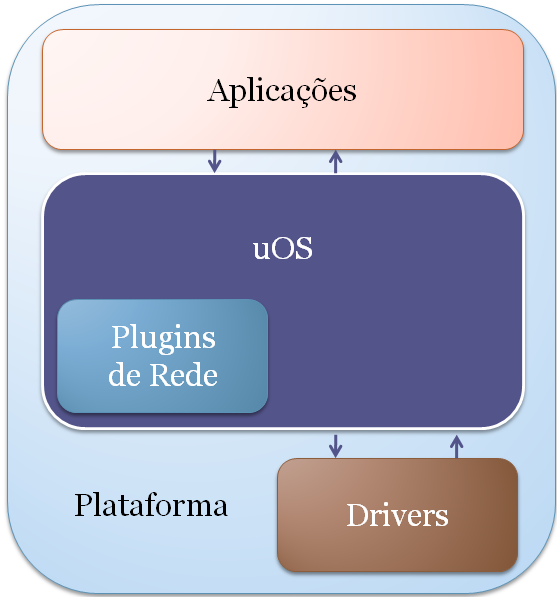
\includegraphics[scale=0.4]{imagens/ecossistemaUbiquitos}
	\caption{Ecossistema do \emph{uOS}.}
	\label{fig:ecossistemaUbiquitos}
\end{figure}

A figura~\ref{fig:ecossistemaUbiquitos} mostra o ecossistema do \emph{middleware}, onde os \emph{plugins}, abstrações para a rede de comunicação, se destacam como um componente dentro do \emph{uOS}. O \emph{uOS}, por sua vez, utiliza os \emph{plugins} para interfacear a comunicação entre aplicações, por meio de \emph{drivers}. No \emph{uOS} destacam-se três camadas: Rede, Conectividade e Adaptabilidade. A camada de Adaptabilidade é responsável pela coordenação de interaçòes feitas por meio do \emph{middleware}. É nessa camada que se encontram o \emph{Device Manager}, responsável pela gerenciamento de dispositivos presentes no ambiente, ou seja, o \emph{Device Manager} é notificado por um radar sobre a entrada ou saída de dispositivos e o \emph{Driver Manager}, responsável por determinar o \emph{driver} de recurso que irá tratar uma chamada recebida pela \emph{Message Engine}. A Figura TODO mostra a arquitetura interna do \emph{uOS}.

No \emph{Driver Manager} foi adicionada uma estrutura em forma de floresta, onde a raiz de cada árvore representa um recurso novo, ou seja, que não é equivalente a nenhum outro recurso. Essa estrutura é inicializada juntamente com o \emph{Driver Manager} com cada tipo básico definidos na Seção~\ref{sec:tiposBasicos} compondo uma nova raiz da estrutura de árvores, definida na Subseção~\ref{subsec:arvoreDeRecursos}. O \emph{Driver Manager} é responsável por manter as relações de equivalência dos recursos, mantendo a consistência de serviços e interfaces e impedindo que ocorra uma referência circular entre recursos equivalentes. Quando um novo recurso é registrado no \emph{middleware}, o \emph{Driver Manager} realiza validações em seu \emph{driver} segundo as relações de quivalência e em seguida o \emph{driver} é adicionado na árvore de equivalência correta. Além de manter essa estrutura, este módulo é responsável por popular a Ontologia do \emph{uOS}. O novo \emph{driver} é adicionado à uma Ontologia por meio da \emph{uOS-Context API}, um conjunto de interfaces que permite a manipulação estrutural e semântica da Ontologia de Contexto do \emph{uOS}~\cite{ozakisbcup2011}. A Figura~\ref{fig:ontologiaUOS} mostra a parte da ontologia que contém as classes dos recursos \emph{Pointer} e \emph{Keyboard}.

\begin{figure}[ht]
	\center
	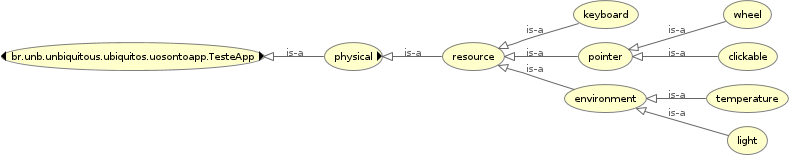
\includegraphics[scale=0.55]{imagens/ontologia}
	\caption{Exemplo de recursos da Ontologia do \emph{uOS}.}
	\label{fig:ontologiaUOS}
\end{figure}

O processo de registro do dispositivo no \emph{middleware} foi modificado. Quando um novo recurso a ser registrado é equivalente a pelo menos um recurso desconhecido, o \emph{Driver Manager} não irá registrá-lo em sua árvore de equivalência enquanto não conhecê-lo. Neste caso, o módulo \emph{Device Manager} é responsável por descobrir esse(s) recurso(s). Após conhecer a interface dos recursos, este módulo irá então registrar cada recurso desconhecido para então registrar o novo recurso na árvore de equivalência.

Para que o \emph{Device Manager} possa descobrir a interface de um determinado recurso desconhecido ele deve procurar o dispositivo que possui este recurso. Dessa forma, o \emph{Device Driver} foi acrescido do serviço \emph{``tellEquivalentDrivers''} que informa a interface de todos os recursos necessários para que o registro no \emph{uOS} possa ocorrer.